\documentclass{beamer}
\usetheme[faculty=econ]{fibeamer}

\usepackage[utf8]{inputenc}
\usepackage[francais]{babel}
\usepackage[T1]{fontenc}
\usepackage{xcolor}

\lstset{
  language=Java,                
  basicstyle=\scriptsize,
  escapeinside={*@}{*@},
  frame=single,
  xleftmargin=2mm,
  xrightmargin=2mm,
  keepspaces=true,
  tabsize=2
}

\newcounter{ctr1}
\title[]{\Large{Développement d'applications modulaires en Java}}
\author[C. Tibermacine]{\large{Chouki~Tibermacine}\\
\small{Chouki.Tibermacine@umontpellier.fr}}
%\institute{Polytech Montpellier}
\date{\tiny{}}

\begin{document}

\begin{frame}
\titlepage
\begin{flushright}

\includegraphics[width=3.5cm]{figs/polytech.png}
\end{flushright}
\end{frame}

\begin{frame}
	\frametitle{Plan de l'ECUE}
	\begin{enumerate}
	{\color{gray} \item (Rappels sur le) Développement d'applications Web avec Java
		\item Modulariser les applications Java avec Spring}
		\item Bien structurer une application Web avec Spring MVC
	{\color{gray}				
		\item Auto-configurer une application Web avec Spring Boot
		\item Sécuriser une application Web avec Spring Security
		\item Gérer des données massives avec Apache Kafka et Spring
		\item Tester une application Web Spring
		\item Écrire des applications Web (API) réactives avec Spring WebFlux}
	\end{enumerate}
\end{frame}

\AtBeginSection[]{% Print an outline at the beginning of sections
  \begin{frame}<beamer>
    \frametitle{Plan du cours}
    % \frametitle{Outline}
    \tableofcontents[currentsection]
    % \tableofcontents
  \end{frame}}

\AtBeginSubsection[]{% Print an outline at the beginning of sections
  \begin{frame}<beamer>
    \frametitle{Plan du cours}
    % \frametitle{Outline}
    \tableofcontents[currentsubsection]
    % \tableofcontents
  \end{frame}}

\section{Introduction à Spring MVC}

\begin{frame}
  \frametitle{Pourquoi Spring MVC~?}
  \begin{itemize}
  \item Gérer la complexité de grandes applications, en séparant les rôles et en les répartissant sur différents composants (gérant le mapping des requêtes, la résolution des vues, la validation des modèles, ...)
  \item Programmation simplifiée par configuration (instanciation automatique, recherche d'instances, ... -- cours Spring DI)
  \item Besoin de développer des applications avec une API REST ou des applications SPA (\textit{Single Page})
  \item Besoin de concevoir des applications indépendamment d'une technologie de templates (HTML, JSP, ...) pour le front-end ou de persistance des données pour le back-end (JDBC, JPA, Hibernate, ...)
  \end{itemize}
\end{frame}

\begin{frame}
	\frametitle{Rappel sur le cycle de vie d'une requête/réponse HTTP}
\begin{tikzpicture}[overlay,remember picture]
	\node[anchor=center,xshift=0pt,yshift=-20pt]
	at (current page.center) {
		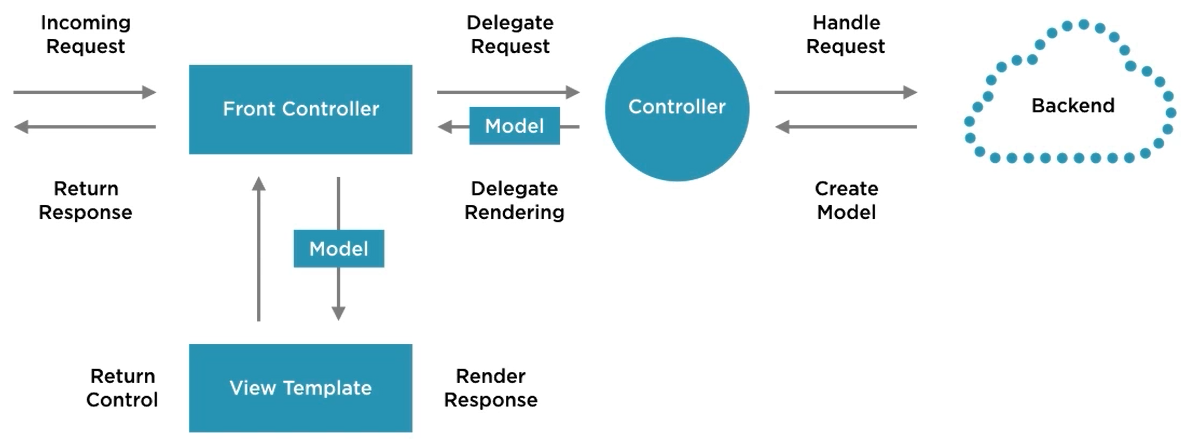
\includegraphics[width=12cm]{img/req_res_lifecycle.png}
	};
\end{tikzpicture}	
\end{frame}

%\begin{frame}
%	\frametitle{Les contrôleurs au cœur des interactions}
%	\begin{tikzpicture}[overlay,remember picture]
%		\node[anchor=center,xshift=0pt,yshift=-20pt]
%		at (current page.center) {
%			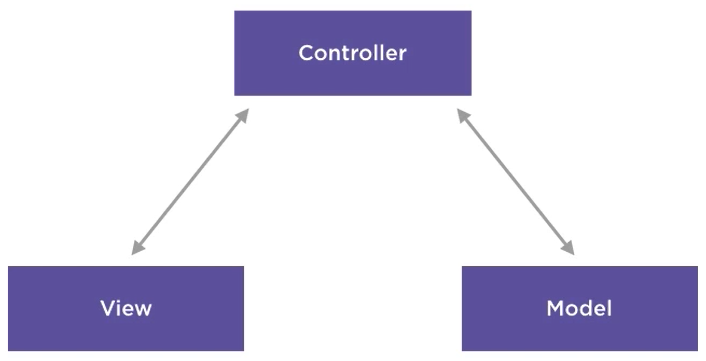
\includegraphics[width=11cm]{img/mvc_pattern.png}
%		};
%	\end{tikzpicture}	
%\end{frame}
%
%\begin{frame}
%	\frametitle{Les contrôleurs au cœur des interactions}
%	\begin{tikzpicture}[overlay,remember picture]
%		\node[anchor=west,xshift=0pt,yshift=-20pt]
%		at (current page.west) {
%			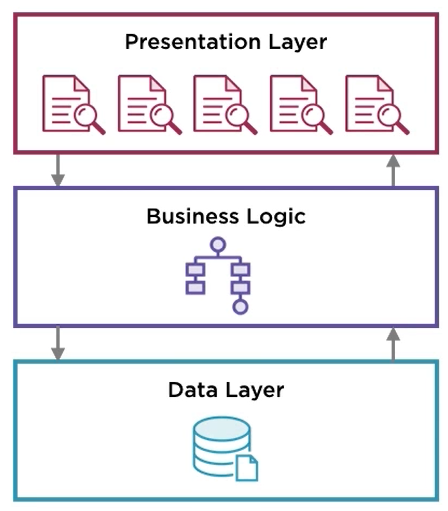
\includegraphics[width=6cm]{img/3_tiers.png}
%		};
%	\end{tikzpicture}
%	\begin{tikzpicture}[overlay,remember picture]
%		\node[anchor=east,xshift=0pt,yshift=-20pt]
%		at (current page.east) {
%			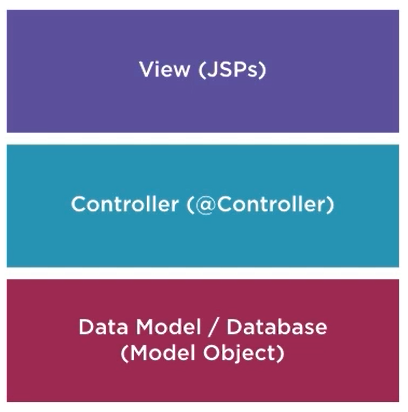
\includegraphics[width=6cm]{img/mvc_tiers.png}
%		};
%	\end{tikzpicture}		
%\end{frame}

\begin{frame}
	\frametitle{Des services derrière les contrôleurs}
	\begin{tikzpicture}[overlay,remember picture]
		\node[anchor=center,xshift=0pt,yshift=-20pt]
		at (current page.center) {
			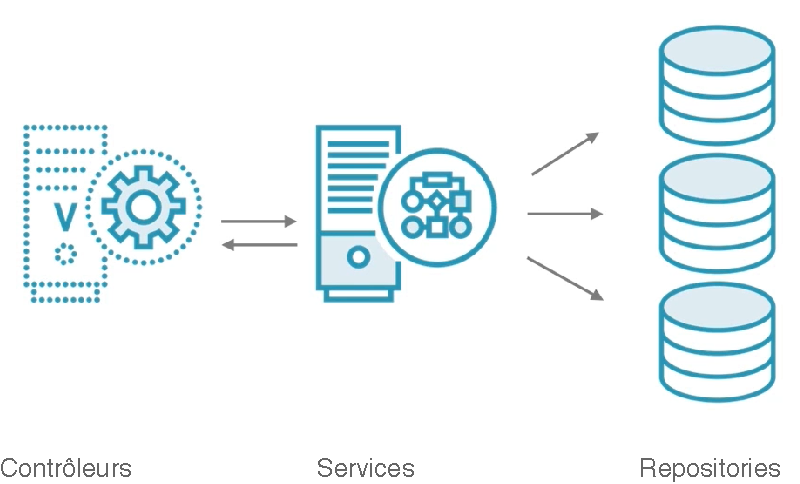
\includegraphics[width=11cm]{img/mvc_services.pdf}
		};
	\end{tikzpicture}	
\end{frame}

\begin{frame}
	\frametitle{Composant ``\textit{Contrôleur}'' dans Spring MVC}
	\begin{itemize}
		\item Gère les requêtes/réponses
		\item Pas de logique métier implémentée dedans
		\item Coordonne les services
		\item Classe annotée par \texttt{@Controller}
		\item Gère les exceptions et le routage vers les vues
	\end{itemize}
\end{frame}

\begin{frame}
	\frametitle{Composant ``\textit{Service}'' dans Spring MVC}
	\begin{itemize}
		\item Classe annotée \texttt{@Service}
		\item Décrit les verbes/actions de l'application
		\item Là où réside la logique métier
		\item Garantit un état cohérent des objets métier
		\item Là où démarrent/s'arrêtent les transactions
	\end{itemize}
\end{frame}

\begin{frame}
	\frametitle{Composant ``\textit{Repository}'' dans Spring MVC}
	\begin{itemize}
		\item Classe annotée \texttt{@Repository}
		\item Décrit les noms (pas les verbes) ou les données de l'application
		\item Là où se déroulent les interactions avec les bases de données
		\item Mapping 1 à 1 avec les objets métier
	\end{itemize}
\end{frame}

\section{Contrôleurs dans Spring MVC}

\begin{frame}
  \frametitle{Que fait un contrôleur ?}
  \begin{itemize}
  \item Interprète et potentiellement transforme les requêtes
  \item Donne accès à la logique métier
  \item Détermine la vue ou le type de réponse
  \item Interprète les exceptions
  \end{itemize}
\end{frame}

\begin{frame}
	\frametitle{\textit{Front Controller Pattern}}
	\begin{itemize}
		\item Spring MVC utilise le patron \textit{Front Controller} pour gérer le front avec les clients
		\item Ce rôle est joué par un objet particulier \textit{Dispatcher Servlet}
		\item Ses missions sont :
		\begin{enumerate}
			\item dispatcher les requêtes  vers des composants \textit{Delegate} gérés par Spring (i.e. \textit{Request Mapping})
			\item résoudre les vues (\textit{View Resolution})
			\item gérer les exceptions (\textit{Exception Handling})
		\end{enumerate}
	\end{itemize}
\end{frame}

\begin{frame}
	\frametitle{\textit{Front Controller Pattern} -suite-}
	\begin{tikzpicture}[overlay,remember picture]
		\node[anchor=center,xshift=0pt,yshift=-20pt]
		at (current page.center) {
			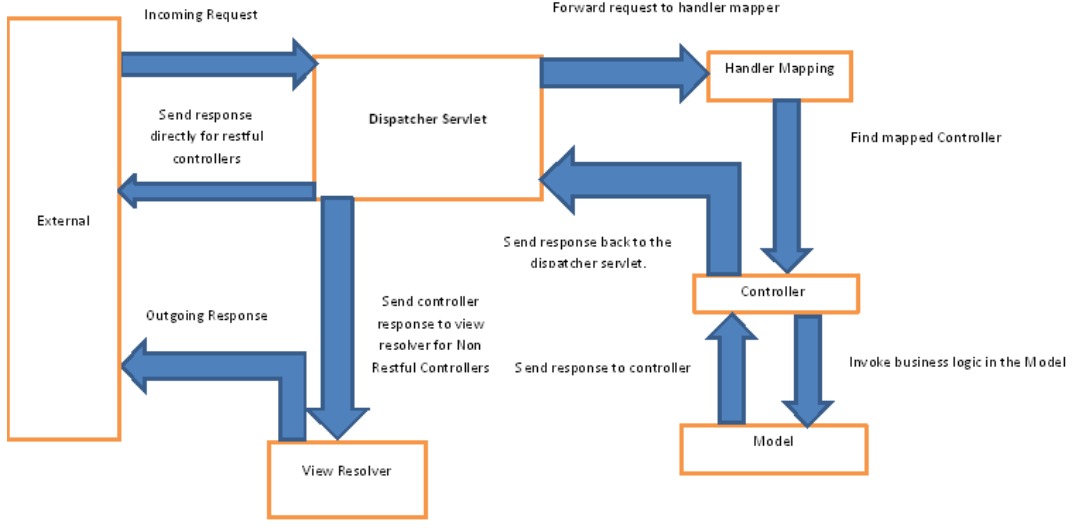
\includegraphics[width=12cm]{img/mvc_with_front_controller.png}
		};
	\end{tikzpicture}	
\end{frame}

\begin{frame}[fragile]
	\frametitle{A vos claviers}
	\begin{itemize}
		\item Créer un projet Gradle (Java et Web) dans IntelliJ
		\item Définir les dépendances suivantes et ajouter le plugin \texttt{org.gretty} au script de build Gradle :
	\end{itemize}
\begin{lstlisting}
dependencies {
  providedCompile('javax.servlet:javax.servlet-api:4.0.1')
  implementation('org.springframework:spring-context:5.3.10')
  implementation('org.springframework:spring-web:5.3.10')
  implementation('org.springframework:spring-webmvc:5.3.10')
  testImplementation('junit:junit:4.13.2')
  testImplementation('org.junit.jupiter:junit-jupiter-api:5.8.1')
  testRuntimeOnly('org.junit.jupiter:junit-jupiter-engine:5.8.1')
}
\end{lstlisting}
Ce script et les classes suivantes sont disponibles sur le dépôt Git (dossier \texttt{code/})
\end{frame}

\begin{frame}[fragile]
	\frametitle{Configurer la \textit{Dispatcher Servlet}}
	1. Définir la classe de configuration (\texttt{AppConfig})~:
\begin{lstlisting}
@EnableWebMvc
@Configuration
@ComponentScan(basePackages = {"fr.poly.mtp.ig5.iwa"})
public class AppConfig  implements WebMvcConfigurer {
 @Override
 public void addViewControllers(
        ViewControllerRegistry registry) {
  registry.addViewController("/").setViewName("index");
 }	
 @Bean
 public ViewResolver viewResolver() {
  InternalResourceViewResolver bean = 
    new InternalResourceViewResolver();		
  bean.setPrefix("/WEB-INF/view/");
  bean.setSuffix(".jsp");		
  return bean;
 }
}
\end{lstlisting}
\end{frame}

\begin{frame}
	\frametitle{Configurer la \texttt{Dispatcher Servlet} -suite-}
	Dans les méthodes de la classe \texttt{AppConfig}, on a indiqué que :
		\begin{itemize}
			\item l'accès à la racine de l'application renvoie à la vue index
			\item les vues seront placées dans le dossier \texttt{WEB-INF/view} et que les noms de vues doivent être tout le temps suffixés par \texttt{.jsp}
		\end{itemize}	
	
\end{frame}

\begin{frame}[fragile]
	\frametitle{Configurer la \texttt{Dispatcher Servlet} -suite-}
	2. Définir une classe d'initialisation~:
\begin{lstlisting}
public class MainWebAppInitializer extends AbstractAnnotationConfigDispatcherServletInitializer {	
	@Override
	protected Class<?>[] getRootConfigClasses() {
		return null;
	}	
	@Override
	protected Class<?>[] getServletConfigClasses() {
		return new Class<?>[] { AppConfig.class };
	}	
	@Override
	protected String[] getServletMappings() {
		return new String[] { "/" };
	}
}
\end{lstlisting}
\end{frame}

\begin{frame}
	\frametitle{A vos claviers}
	\begin{itemize}
		\item Ajouter un fichier \texttt{index.jsp} dans le dossier \texttt{webapp/WEB-INF/view/}
		\item Mettre un lien dans cette page JSP qui pointe vers une vue (registration.jsp) qui fournit un formulaire HTML dans lequel on peut saisir les informations concernant un utilisateur à inscrire sur un site Web
		\item On écrira plus tard la servlet \texttt{Controller} qui donne accès à cette vue et qui va aussi traiter les données du formulaire
		\item Pour déployer l'application, exécuter la tâche gretty/appRun, en allant dans la \textit{tool window} ``\textit{gradle}'' sur IntelliJ (en l'ouvrant depuis la barre latérale droite), puis \texttt{Tasks}, puis \texttt{gretty}, puis clique bouton-droit sur \texttt{appRun}, puis \texttt{Run}
	\end{itemize}
\end{frame}

\begin{frame}
	\frametitle{Annotations pour les contrôleurs de vues}
	\begin{itemize}
		\item Annotations utilisées pour marquer les classes qui vont s'exécuter à la réception de requêtes HTTP
		\item Ces classes doivent être placées dans le package indiqué dans \texttt{@ComponentScan} dans la classe \texttt{AppConfig}, ou l'un de ses sous-packages (un sous-package \texttt{controllers} par ex.)
		\item Dans ces classes, on déclare les méthodes qui vont recevoir chaque type de requête (Get, Post, ...) pour une route donnée
		\item Ces méthodes seront annotées \texttt{@GetMapping}, \texttt{@PostMapping} ou avec l'annotation générique \texttt{@RequestMapping}
		\item Les routes sont indiquées dans ces annotations 
	\end{itemize}
\end{frame}


\begin{frame}[fragile]
	\frametitle{Exemple de contrôleur de vue}
\begin{itemize}
	\item Une classe RegistrationController
\begin{lstlisting}
package fr.poly.mtp.ig5.iwa.controller;
// import ... 
@Controller
public class RegistrationController {
	@GetMapping("registration")
	public String getRegistration() {
		return "registration";
	}
	@PostMapping("registration")
	public String addRegistration() {
		// ...
		return "registration";
	}
}
\end{lstlisting}
\end{itemize}
La première méthode permet de diriger vers la vue \texttt{registration}(.jsp) si l'utilisateur envoie une requête Get ``\$\{context.path\}/registration'' (\$\{context.path\}=nom projet IDEA)
\end{frame}

\begin{frame}
\frametitle{Annotations pour les contrôleurs de vues -suite-}
\begin{itemize}
		\item Les méthodes des contrôleurs peuvent déclarer des paramètres 
		\item Ces paramètres peuvent être rattachés directement à des données transmises par les vues (champs dans un formulaire, par exemple)
		\item Ces paramètres sont annotés \texttt{@ModelAttribute}
	\end{itemize}
\end{frame}

\begin{frame}[fragile]
	\frametitle{Exemple d'attribut de modèle}
	\begin{itemize}
		\item Un objet (bean) de type \texttt{Registration} (une nouvelle classe à écrire, qui fait partie du modèle) est passé en paramètre
\begin{lstlisting}
@GetMapping("registration")
public String getRegistration(@ModelAttribute("registration") Registration registration) {
	return "registration";
}	
@PostMapping("registration")
public String addRegistration(@ModelAttribute("registration") Registration registration) {
	System.out.println("Registration : "+registration.getName());
	return "process_registration";
}
\end{lstlisting}
	\end{itemize}
\end{frame}

\begin{frame}[fragile]
	\frametitle{Lier les vues aux modèles}
\begin{lstlisting}
<%@ page contentType="text/html;charset=UTF-8" 
         language="java" %>
<%@taglib prefix="form" 
          uri="http://www.springframework.org/tags/form" %>
<html>
 <head><title>Signing up a user</title></head>
<body>
 <h2>Signing up a user</h2>
 <form:form modelAttribute="registration">
  <div>
  Name:
  <form:input path="name"/>
  ...
  </div>
  ...
 </div>
 </form:form>
</body>
</html>
\end{lstlisting}
\end{frame}

\begin{frame}
	\frametitle{Lier les vues aux modèles -suite-}
	Dans l'exemple précédent :
	\begin{enumerate}
		\item Déclarer dans la vue l'utilisation d'une librairie de balises (\textit{taglib}) de Spring et lui donner un identifiant, qui servira comme préfixe
		\item Utiliser ces balises (en préfixant les balises HTML du préfixe précédent -- \texttt{form} dans l'exemple)
		\item Déclarer un attribut \texttt{modelAttribute} ayant comme valeur un bean qui servira comme objet du modèle
		\item Déclarer dans les éléments (champ d'un formulaire par exemple) le lien entre la valeur de cet élément et la valeur d'une propriété du bean (\texttt{path="name"} dans l'exemple)
	\end{enumerate}
\end{frame}

\begin{frame}
	\frametitle{Lier les vues aux modèles -suite-}
	\begin{itemize}
\item Dans l'exemple précédent, nous avions un bean dont l'id est \texttt{registration}
\item Ajouter dans votre projet IntelliJ une classe Registration avec une propriété (attribut avec des accesseurs publics) \texttt{name}
\item Tester votre application
\item Ajouter d'autres champs dans le formulaire (email, ...)
\item Compléter le code de la classe du bean
\item Tester dans le contrôleur la bonne réception des données saisies dans le formulaire
	\end{itemize}
\end{frame}

\section{Vues dans Spring MVC}

\begin{frame}
  \frametitle{\textit{View Resolver}}
\begin{tikzpicture}[overlay,remember picture]
	\node[anchor=center,xshift=0pt,yshift=0pt]
	at (current page.center) {
		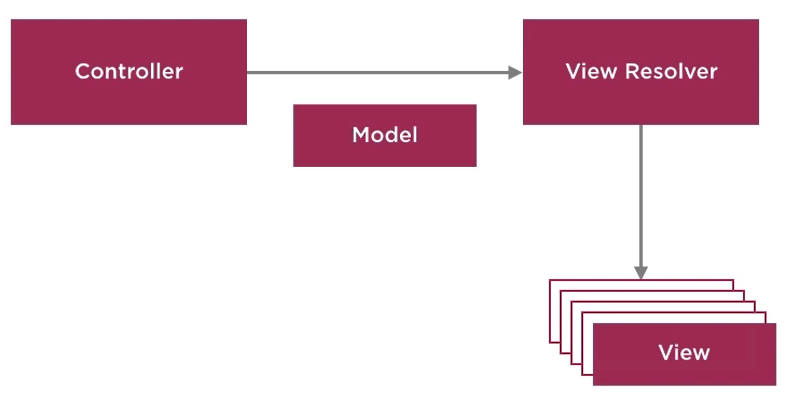
\includegraphics[width=12cm]{img/view_resolver.png}
	};
\end{tikzpicture}  
  \begin{itemize}
  	\vspace{5cm}
  \item Un objet utilisé par le contrôleur pour choisir les vues
  \end{itemize}
\end{frame}

\begin{frame}[fragile]
	\frametitle{Dans les exemples précédents}
	\begin{itemize}
		\item On a créé précédemment un \textit{View Resolver} dans \texttt{AppConfig}

\begin{lstlisting}
...
public class AppConfig  implements WebMvcConfigurer {	
	...
	@Bean
	public ViewResolver viewResolver() {
		InternalResourceViewResolver bean = new InternalResourceViewResolver();		
		bean.setPrefix("/WEB-INF/view/");
		bean.setSuffix(".jsp");		
		return bean;
	}
}
\end{lstlisting}
\item Il choisit les vues dans le dossier \texttt{WEB-INF/view/} et ce sont des fichiers dont le nom est constitué du nom de la vue + ".jsp" (l'utilisateur ne verra pas .jsp)
	\end{itemize}
\end{frame} 

\begin{frame}[fragile]
	\frametitle{Résoudre les fichiers statiques}
	\begin{itemize}
		\item Pour les fichiers statiques (HTML, CSS et JS, PDF, ...), on peut les placer dans un dossier WEB-INF/static/ (ensuite un sous-dossier par type de fichier : html/ js/ ...) et ensuite :
\begin{lstlisting}
public void addResourceHandlers(ResourceHandlerRegistry registry) {
 registry.addResourceHandler("/*.html")
 .addResourceLocations("/WEB-INF/static/html/");
 registry.addResourceHandler("/images/**")
 .addResourceLocations("/WEB-INF/static/html/images/");
}
\end{lstlisting}		
	\end{itemize}
\end{frame} 

\begin{frame}
	\frametitle{Internationalisation \textit{I18N} des vues}
	\begin{itemize}
		\item Support pour d'autres langues/locales (anglais, espagnol, ...)
		\item Basée sur les intercepteurs (\textit{Interceptors})
		\item Procédure à suivre~:
		\begin{enumerate}
			\item Définir un \textit{locale resolver} et indiquer la locale par défaut
			\item Définir et enregistrer un intercepteur de changement de locale
			\item Créer des fichiers .properties qui contiennent les mots/phrases (messages) dans différentes langues
			\item Remplacer dans les pages JSP le texte par des balises spéciales qui déclenchent ce système d'internationalisation
		\end{enumerate}
		\item Étapes expliquées et illustrées dans les diapos suivantes
	\end{itemize}
\end{frame} 

\begin{frame}[fragile]
	\frametitle{Configuration de la locale}
	\begin{itemize}
		\item Config de la locale par défaut dans un \textit{Locale Resolver} à ajouter dans la classe \texttt{AppConfig}~:
\end{itemize}

\begin{lstlisting}
@Bean
public LocaleResolver localeResolver() {
 SessionLocaleResolver slr=new SessionLocaleResolver();
 slr.setDefaultLocale(Locale.FRANCE);
 return slr;
}
\end{lstlisting}
	\begin{itemize}
		
\item Ajouter la source des messages (toujours dans la même classe)~:
\end{itemize}

\begin{lstlisting}
@Bean
public ReloadableResourceBundleMessageSource messageSource() {
	ReloadableResourceBundleMessageSource resource = new ReloadableResourceBundleMessageSource();
	resource.setBasename("WEB-INF/languages/messages");
	resource.setDefaultEncoding("UTF-8");
	return resource; }
\end{lstlisting}
\end{frame} 

\begin{frame}[fragile]
	\frametitle{Configuration de la locale -suite-}
	\begin{itemize}
		\item Config de l'intercepteur de changement de locale (\texttt{AppConfig}):
\end{itemize}

\begin{lstlisting}
@Bean
public LocaleChangeInterceptor localeChangeInterceptor() {
 LocaleChangeInterceptor lci=new LocaleChangeInterceptor();
 lci.setParamName("lang");
 return lci;
}
\end{lstlisting}
	\begin{itemize}

\item[] Ici, on indique que la locale doit être lue dans le paramètre ``\texttt{lang}" de la requête (\texttt{?lang=us}, par ex)
\item Enregistrement de l'intercepteur :
	\end{itemize}

\begin{lstlisting}
public void addInterceptors(InterceptorRegistry registry) {
  registry.addInterceptor(localeChangeInterceptor());
}
\end{lstlisting}
\end{frame} 

\begin{frame}[fragile]
	\frametitle{Implémenter les messages dans différentes locales}
	\begin{itemize}
		\item Créer dans un dossier \texttt{WEB-INF/languages/} un fichier \texttt{messages.properties} avec le contenu suivant :
\begin{lstlisting}
#labels
name=Nom
email=Courriel
\end{lstlisting}
ça sera le fichier pour la locale par défaut (le français)
\item Pour d'autres langues, créer, dans le même dossier, des fichiers \texttt{messages\_us.properties} (pour l'anglais), \texttt{messages\_es.properties} (pour l'espagnol), ...
	\end{itemize}
\end{frame}

\begin{frame}[fragile]
	\frametitle{Utiliser les locales}
	\begin{itemize}
		\item Dans une page JSP, déclarer la taglib~:
\begin{lstlisting}
<%@ taglib prefix="spring"
    uri="http://www.springframework.org/tags" %>
\end{lstlisting}
\item Remplacer le texte à internationaliser par des balises issues de la taglib
\item Exemple : remplacer le label \texttt{Nom} par~:
\begin{lstlisting}
<spring:message code="name"/>
\end{lstlisting}
Selon la langue choisie par l'utilisateur, le bon fichier .properties sera lu pour obtenir la valeur du message "name"
	\end{itemize}
\end{frame}

\begin{frame}
	\frametitle{Quels solveurs de locales~?}
	\begin{itemize}
		\item Spring fournit un certain nombre de solveurs concrets de locales
		\item Dans l'exemple précédent, nous avons utilisé un \texttt{SessionLocaleResolver}, qui utilise l'attribut \texttt{locale} dans la session utilisateur (locale valable toute une session)
		\item Autres solveurs~:
		\begin{itemize}
			\item \texttt{AcceptHeaderLocaleResolver} utilise l'entête HTTP de la requête "accept-language"
			\item \texttt{FixedLocaleResolver} retourne une locale par défaut fixe
			\item \texttt{CookieLocaleResolver} utilise une locale stockée dans un cookie
		\end{itemize}
	\end{itemize}
\end{frame} 

\begin{frame}
	\frametitle{PRG (\textit{Post-Redirect-Get}) Pattern}
\begin{tikzpicture}[overlay,remember picture]
	\node[anchor=center,xshift=0pt,yshift=0pt]
	at (current page.center) {
		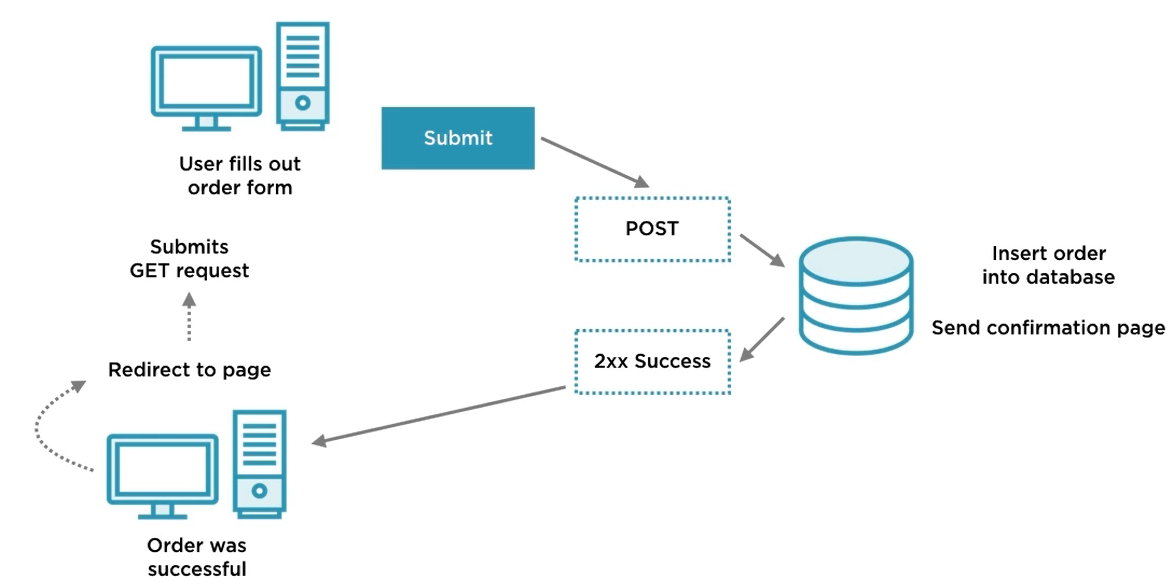
\includegraphics[width=12cm]{img/PRG_Pattern.png}
	};
\end{tikzpicture}
\begin{itemize}
	\vspace{5.5cm}
	\item Objectif : après avoir traité un POST, on ne renvoie pas vers la vue d'origine ; on répond par une redirection pour que le navigateur fasse un Get de la vue (données sur la vue effacées)
\end{itemize}
\end{frame} 

\begin{frame}[fragile]
	\frametitle{PRG (\textit{Post-Redirect-Get}) Pattern -suite-}
\begin{itemize}
	\item Remplacer dans le contrôleur (le \texttt{return})
\begin{lstlisting}
@PostMapping("registration")
public String addRegistration(@ModelAttribute("registration") Registration registration) {
	System.out.println("Name: "+registration.getName());
	return "registration";
}
\end{lstlisting}	

\item par :
\begin{lstlisting}
	@PostMapping("registration")
	public String addRegistration(@ModelAttribute("registration") Registration registration) {
		System.out.println("Name: "+registration.getName());
		return "redirect:registration";
	}
\end{lstlisting}
\item Tester avant et après
\end{itemize}
\end{frame} 

\section{Templates de vues \textit{Thymeleaf}}

\begin{frame}
	\frametitle{Pourquoi \textit{Thymeleaf} ?}
	\begin{itemize}
		\item Pour beaucoup de développeurs, avoir du JSP dans son application Web est considéré comme une dette technique
		\item On considère que JSP doit être remplacé par des technologies plus modernes de templating
		\item \textit{Thymeleaf} est un framework de templating, qui s'intègre bien avec Spring
		\item De nos jours, on utilise ce genre de frameworks en combinaison avec des framework de front-end comme Angular, React, Vue, ...
	\end{itemize}
\end{frame} 

\begin{frame}[fragile]
	\frametitle{Dépendances à \textit{Thymeleaf}}
	\begin{itemize}
		\item Ajouter dans le build.gradle la dépendance:
	\end{itemize}		
\begin{lstlisting}
implementation("org.thymeleaf:thymeleaf-spring5:3.0.11.RELEASE")
\end{lstlisting}
	\begin{itemize}
		\item Tester le téléchargement des bibliothèques :
		\begin{itemize}
			\item Sur IntelliJ, dans la tool-window Gradle, cliquer sur le bouton d'actualisation du projet 
			\item Aller ensuite dans l'explorateur du projet et ouvrir le dossier ``Bibliothèques externes'' (``\textit{External Libraries}'') pour vérifier si de nouveaux JAR Thymeleaf ont été ajoutés
		\end{itemize} 
	\end{itemize}
\end{frame}

\begin{frame}[fragile]
	\frametitle{\textit{Template Resolver}}
	\begin{itemize}
		\item Dans le configurateur des contrôleurs et des solveurs de vues/locales, on ajoute une méthode qui retourne un bean de type \texttt{TemplateResolver} (différent d'un \textit{View Resolver})~:
	\end{itemize}

\begin{lstlisting}
@Bean
public SpringResourceTemplateResolver templateResolver() {
	SpringResourceTemplateResolver templateResolver = new SpringResourceTemplateResolver();
	templateResolver.setApplicationContext(appContext);
	templateResolver.setPrefix("/WEB-INF/view/");
	templateResolver.setSuffix(".html");
	return templateResolver;
}
\end{lstlisting}
\begin{itemize}
\item Ajouter l'attribut (auto-injecté) \texttt{appContext} dans la classe~:
\end{itemize}
\begin{lstlisting}
@Autowired
private ApplicationContext appContext;
\end{lstlisting}
	
\end{frame} 

\begin{frame}[fragile]
	\frametitle{\textit{Template Engine}}
	\begin{itemize}
		\item Moteur nécessaire pour produire des vues à partir de templates Thymeleaf
		\item Ajouter dans la même classe une méthode qui retourne un bean de type \texttt{TemplateEngine}~:
\begin{lstlisting}
@Bean
public SpringTemplateEngine templateEngine() {
	SpringTemplateEngine templateEngine = 
		new SpringTemplateEngine();
	templateEngine.setTemplateResolver(
		templateResolver());
	templateEngine.setEnableSpringELCompiler(true);
	return templateEngine;
}
\end{lstlisting}
Noter la référence vers le \textit{Template Resolver}
	\end{itemize}
\end{frame} 

\begin{frame}[fragile]
	\frametitle{\textit{View Resolver}}
	\begin{itemize}
		\item Ajouter un \textit{View Resolver} dans la même classe que précédemment
\begin{lstlisting}
@Bean
public ViewResolver thymeleafResolver() {
	ThymeleafViewResolver viewResolver = new ThymeleafViewResolver();
	viewResolver.setTemplateEngine(templateEngine());
	viewResolver.setOrder(0);
	return viewResolver;
}
\end{lstlisting}
		\item setOrder() doit indiquer une valeur inférieur à celle utilisée dans le view resolver de JSP (setOrder(1) pour le view resolver de JSP et setOrder(0) pour celui de Thymeleaf)
		\item Dans une vraie app, il vaut mieux enlever le view resolver de JSP (au lieu de faire cohabiter les 2)
	\end{itemize}
\end{frame} 

\begin{frame}[fragile]
	\frametitle{Définir des templates HTML avec Thymeleaf}
	\begin{itemize}
		\item Créer une page HTML, (\texttt{home.html} par exemple) dans le dossier \texttt{WEB-INF/view}~:
\begin{lstlisting}
<!DOCTYPE html>
<html lang="en" xmlns:th="http://www.thymeleaf.org">
<head>
 <meta charset="UTF-8">
 <title>Accueil Thymeleaf</title>
</head>
<body>
 <h1>Accueil Thymeleaf</h1>
 <p th:text="${message}"></p>
</body>
</html>
\end{lstlisting}
\item Noter le \texttt{xmlns:th} au début et l'attribut
 \texttt{th:text}
 \item D'où provient l'objet \texttt{message} utilisé ci-dessus~?
	\end{itemize}
\end{frame}

\begin{frame}[fragile]
	\frametitle{Contrôleur pour les requêtes vers cette vue}
	\begin{itemize}
		\item L'objet \texttt{message} dans cet exemple provient du modèle, mis à disposition par le contrôleur de requêtes HTTP vers cette vue~:
		
\begin{lstlisting}
@GetMapping("home")
public String getRegistration(Map<String, Object> model) {
	model.put("message","Fantastic Thymeleaf!!!");
	return "home";
}
\end{lstlisting}
\item C'est juste une chaîne de caractères ici
	\end{itemize}
Plus de détails sur Thymeleaf ici~: \url{https://www.thymeleaf.org/}

Comme vous pouvez le constater, les vues précédentes (JSP) ne sont plus accessibles (il y a une manip à faire pour faire cohabiter JSP et Thymeleaf, mais on ne le fera pas ici. Choisir l'un des 2)

\end{frame} 

\section{Validation des beans des modèles}

\begin{frame}
	\frametitle{Validation des beans}
	\begin{itemize}
		\item Besoin de garantir des modèles valides dans les applications
		\item Même si certaines validations sont possibles en JavaScript côté client, il vaut mieux vérifier les données côté serveur (si jamais JS est désactivé sur le navigateur du client)
		\item Au départ, il y avait l'interface Validator, puis plusieurs JSR ont fait évoluer ce système de validation (dernière en date, JSR 380 pour Java8+ : API javax.validation)
		\item L'idée de base est de~:
		\begin{enumerate}
			\item contraindre les valeurs des propriétés de beans (objets du modèle)
			\item faire apparaître des messages d'erreur en cas de violation de ces contraintes 
		\end{enumerate}
	\end{itemize}
\end{frame} 

\begin{frame}[fragile]
	\frametitle{Configuration de la validation}
	\begin{itemize}
		\item Mise en place des dépendances (sur Gradle)
\begin{lstlisting}
implementation("org.hibernate.validator:hibernate-validator:6.0.2.Final")
\end{lstlisting}
		hibernate-validator est l'implémentation de référence de l'API de validation (javax.validation). Elle n'est pas liée à l'API de persistance de Hibernate
		\item Tester la présence de la bibliothèque dans votre projet
	\end{itemize}
\end{frame} 

\begin{frame}
	\frametitle{Mise en place de la validation}
	\begin{itemize}
		\item Annoter les attributs des objets du modèle
		\item Quelles annotations ?
		\begin{itemize}
			\footnotesize
			\item \texttt{@NotEmpty}, \texttt{@NotNull}, \texttt{@AssertTrue}
			\item \texttt{@Size(min = 10, max = 200,\\ message 
				= "About Me must be between 10 and 200 chars")\\
				private String aboutMe;}
			\item \texttt{@Email(message = "Email should be valid")\\
				private String email;}
			\item \texttt{@Min(value=18, message="Age should not be < 18")\\
				@Max(value=150, message="Age should not be > 150")\\
				private int age;}
			\normalsize
		\end{itemize}
		\item Ensuite, annoter avec \texttt{@Valid} les paramètres des méthodes des contrôleurs via lesquels transitent les objets du M
		\item Enfin, il faudra gérer les éventuelles erreurs
		
	\end{itemize}
\end{frame} 

\begin{frame}[fragile]
	\frametitle{Gestion des erreurs}
	\begin{itemize}
		\item Dans une app Web, on va (dans une page JSP):
		\begin{itemize}
			\item 1. prévoir un bloc qui va apparaître en cas d'erreur (\texttt{<form:errors>} à l'intérieur de \texttt{<form>})
\begin{lstlisting}
<form:errors path="*" cssClass="errorblock" 
             element="div"/>
\end{lstlisting}
			En ayant prévu une classe CSS \texttt{errorblock} (ou utiliser des classes de frameworks CSS comme Bootstrap)
			\item[-] Pour le faire avec Thymeleaf (ignorer la partie Spring Boot)~:\\
			\footnotesize
			\url{https://spring.io/guides/gs/validating-form-input/}
			\normalsize
		\end{itemize}
		\item[-]Dans l'exemple précédent, on va marquer:
		\begin{itemize}
			\item l'attribut \texttt{email} de la classe \texttt{Registration} par l'annotation~:\\ \texttt{@Email(message="Email is not well-formed")}
			\item et l'attribut \texttt{name} par l'annotation~:\\
			\texttt{@NotEmpty(message="Name must not be empty")}
		\end{itemize}
	\end{itemize}
\end{frame}

\begin{frame}[fragile]
	\frametitle{Gestion des erreurs -suite-}
		\begin{itemize}
			\item 2. affiner le contrôleur/solveur de vues~:
		
\begin{lstlisting}
@PostMapping("registration")
public String addRegistration(@Valid 
      @ModelAttribute("registration") 
      Registration registration,
      BindingResult result) {
	if(result.hasErrors()) {return "registration";}
	System.out.println(registration.getName());
	return "redirect:registration";
}
\end{lstlisting}
		
		Noter ici :
		\begin{itemize}
			\item l'utilisation de l'annotation \texttt{@Valid}
			\item le second paramètre de la méthode, de type \texttt{BindingResult}
			\item le test \texttt{hasErrors()} et le retour à la vue (sans utilisation du patron PRG -- \texttt{redirect:})
		\end{itemize}
	\end{itemize}
\end{frame} 

\begin{frame}
	\frametitle{Personnaliser les messages d'erreur}
	\begin{itemize}
		\item Il est possible d'utiliser l'internationalisation pour personnaliser les messages d'erreurs
		\item Dans les fichiers \texttt{messages.properties} vus précédemment, on va ajouter~:\\
		NotEmpty.registration.name=Le champ nom ne doit pas $\backslash$u00EAtre vide
		\item[-]Ici, \texttt{registration} correspond à l'id du bean concerné par l'annotation et \texttt{name} est le nom de la propriété du bean
		\item[-]le caractère 'ê' est remplacé ici par son code Unicode. Il existe des plugins Gradle (\textit{native2ascii}, par ex), qui peuvent gérer les caractères avec accents dans des fichiers .properties
	\end{itemize}
\end{frame} 

\section{Services REST avec Spring MVC}
\begin{frame}
	\frametitle{Services REST}
	\begin{itemize}
		\item Au lieu de servir des vues (pages HTML), une application Spring MVC peut servir des données, via des services REST (une alternative à JAX-RS de Java Enterprise -- Jakarta EE)
		\item Par défaut, les services retournent des objets sérialisées comme données JSON
		\item Très simple à mettre en place~:
		\begin{itemize}
			\item Utiliser l'annotation \texttt{@RestController} pour marquer une classe contrôleur de services REST
			\item Utiliser les annotations déjà vues (\texttt{@GetMapping}, ...) pour marquer les méthodes de cette classe (les \textit{endpoints} du service)
			\item Utiliser l'annotation \texttt{@RequestParam(value="...",defaultValue="...")} pour marquer les paramètres des méthodes
			\item retourner des objets dans ces méthodes
		\end{itemize}
	\end{itemize}
\end{frame} 

\begin{frame}[fragile]
	\frametitle{Exemple de service REST avec Spring}
	\begin{itemize}
		\item Définir une classe (de beans) nommée User avec les propriétés \texttt{prenom}, \texttt{nom} et \texttt{age} (ou renommer Registration en User)
		\item Définir une classe \texttt{UserController}, annotée \texttt{@RestController}
		\item Y ajouter une méthode \texttt{getUser()} annotée \texttt{@GetMapping("/user")}
		\item[]Cette méthode crée un objet User et le retourne
		\item Ajouter 3 paramètres à cette méthode pour chaque propriété de beans User
		\item[-]Exemple de paramètre~:\\
		@RequestParam(value="prenom",defaultValue="Elon")\\ String prenom
	\end{itemize}
\end{frame} 

\begin{frame}[fragile]
	\frametitle{Mapping objets Java vers données JSON}
	\begin{itemize}
		\item Dans le script de build de Gradle, ajouter les dépendances suivantes vers le mapper objets/JSON~:
	\end{itemize}
\begin{lstlisting}
implementation("com.fasterxml.jackson.core:jackson-core:2.11.2")
implementation("com.fasterxml.jackson.core:jackson-databind:2.11.2")
\end{lstlisting}
	\begin{itemize}
		\item Tester le service REST précédent~:
		\url{http://localhost:8080/votreprojet/user}
		\url{http://localhost:8080/votreprojet/user?prenom=Ian}
	\end{itemize}
\end{frame} 

\begin{frame}[fragile]
	\frametitle{Services REST de type POST, PUT, ...}
	\begin{itemize}
		\item Pour les services REST de type Post, Put, Delete, ... le paramètre peut être un simple objet (User dans notre exemple)
	\end{itemize}
\begin{lstlisting}
@PostMapping("/user")
public User postUser(@RequestBody User user) {
	System.out.println("Prenom : "+user.getPrenom());
	return user;
}
\end{lstlisting}
	\begin{itemize}
		\item Cet objet est construit automatiquement par le mapper (prévoir un constructeur vide sans params) à partir des données de la requête HTTP
		\item Pour tester ce service, on peut utiliser \texttt{curl} ou des outils de test d'app Web comme \textit{Postman}
	\end{itemize}
	Écrire maintenant une page HTML avec un script jQuery qui interroge le serveur pour récupérer les données d'un utilisateur (service GET précédent) et les affiche dans la page 
\end{frame} 

\section{Conclusion}
\begin{frame}
	\frametitle{\textit{Wrap-up}}
	\begin{itemize}
		\item Développement d'app Web bien structurées, avec du typage statique à la Java pour plus de vérifications à la compilation
		\item Contrôleurs au coeur du framework Spring MVC
		\item Solveurs de vues et templating avec Thymeleaf
		\item Validation des modèles avec javax.validation
		\item Services REST très simples à mettre en place avec Spring MVC
		\item Aller plus loin en simplifiant plein de configurations avec Spring Boot (prochain cours)
	\end{itemize}
\end{frame} 

\begin{frame}
	\frametitle{Références biblio}
	\begin{itemize}
		\item Site Web de Spring~: \url{https://spring.io/learn}
		\item Tutoriels sur Pluralsight et Baeldung
		\item Livres sur le sujet~:\\
		\url{https://hackr.io/blog/spring-books}
	\end{itemize}
\end{frame} 


\begin{frame}
	\begin{tikzpicture}[overlay,remember picture]
		\node[anchor=center,xshift=0pt,yshift=0pt]
		at (current page.center) {
			
\includegraphics[width=4cm]{img/question.jpg}
		};
	\end{tikzpicture}
\end{frame}

\end{document}
